\documentclass[11pt]{article}
\usepackage[a4paper,top=22mm,bottom=23mm,left=25mm,right=25mm]{geometry}
\usepackage{fontspec,amsmath,amssymb,amsthm,graphicx,xcolor}
\definecolor{deep}{HTML}{194F5C}
\linespread{1.17}
\setlength{\emergencystretch}{2em}
\raggedbottom
\usepackage[unicode,hidelinks,pdftitle={交替粒子链的一个高斯势反例与里斯势的能量下界}]{hyperref}
% Shared by en/paper.tex and zh/paper.tex. Compile within each language directory.
\newcommand*{\ResearchAuthor}{Codex (OpenAI AI model)}
\newcommand*{\CorrespondingAuthor}{guowei jiang}

\hypersetup{pdfauthor={\ResearchAuthor; Corresponding author: \CorrespondingAuthor}}
\setmainfont{Noto Serif CJK SC}[ItalicFont={Noto Serif CJK SC},ItalicFeatures={FakeSlant=0.16}]
\XeTeXlinebreaklocale "zh"
\XeTeXlinebreakskip=0pt plus 1pt
\setlength{\parindent}{2em}
\renewcommand{\abstractname}{摘要}
\renewcommand{\proofname}{证明}
\renewcommand{\refname}{参考文献}
\theoremstyle{definition}
\newtheorem{theorem}{定理}
\newtheorem{proposition}[theorem]{命题}
\newcommand{\Z}{\mathbb Z}
\newcommand{\R}{\mathbb R}
\newcommand{\dd}{\,\mathrm d}
\title{\bfseries\color{deep}交替粒子链的一个高斯势反例\\与里斯势的能量下界}
\author{\ResearchAuthor\\[2pt]\small 通讯作者：\CorrespondingAuthor}
\date{2026 年 11 月 25 日}
\begin{document}
\maketitle
\begin{abstract}
考虑两类粒子交替排列、密度固定的一维链。对高斯相互作用势，我们构造了一个每周期含四个粒子的构型，其能量严格低于等距链。这给出了 Bétermin、Knüpfer 和 Nolte 期刊论文中猜想 2.7 的反例。在一段高斯势的尺度参数范围内，从等距构型出发，还存在一个使能量严格下降的位移方向。对由距离的衰减指数函数按正测度叠加得到的势，我们直接证明了一个可由已有尖界面模型能量界推出的区间估计。该估计表明等距链是唯一达到最低能量的构型，并适用于一切 $p>0$ 的逆幂势 $r^{-p}$，覆盖了同一论文评注 2.6 提出的整个指数范围。
\end{abstract}

\section{能量定义与两个待检验的命题}
固定偶数 $N$ 和周期长度 $L$。粒子位置满足 $x_{i+N}=x_i+L$、$x_i<x_{i+1}$，并取 $x_0=0$。相邻粒子的平均间距为 $\ell=L/N$。用 $\sigma_i=(-1)^i$ 标记两类粒子。沿用文献\cite{BKN}的两体势约定 $f_{11}=f_{22}=-f$、$f_{12}=f$，构型 $X$ 的平均每粒子能量为
\begin{equation}\label{eq:energy}
 E_f(X)=-\frac1N\sum_{i=0}^{N-1}\sum_{j\in\Z,\ j\ne i}
                 \sigma_i\sigma_j f(|x_i-x_j|).
\end{equation}
这一符号约定使同类粒子对的能量取负值。式\eqref{eq:energy}遵循原文的归一化方式，按照有序粒子对计数。对于仅条件收敛的核，从参考粒子出发，分别向右和向左按距离递增的顺序求和。用 $U$ 表示等距构型 $x_i=i\ell$。

文献\cite{BKN}的猜想 2.7 认为，若 $f(r)=F(r^2)$ 且 $F$ 完全单调，则在任意尺度下，$U$ 都是唯一使能量最低的构型。下文使用的高斯势属于这一类。文献\cite{BKN}的定理 2.4 已证明，对逆幂势 $f(r)=r^{-p}$，当 $p\ge p_0\simeq0.655$ 时，等距构型的能量最低。该文评注 2.6 提出，这一结果可能适用于每一个 $p>0$。下文分别考察这两个命题。

\begin{center}
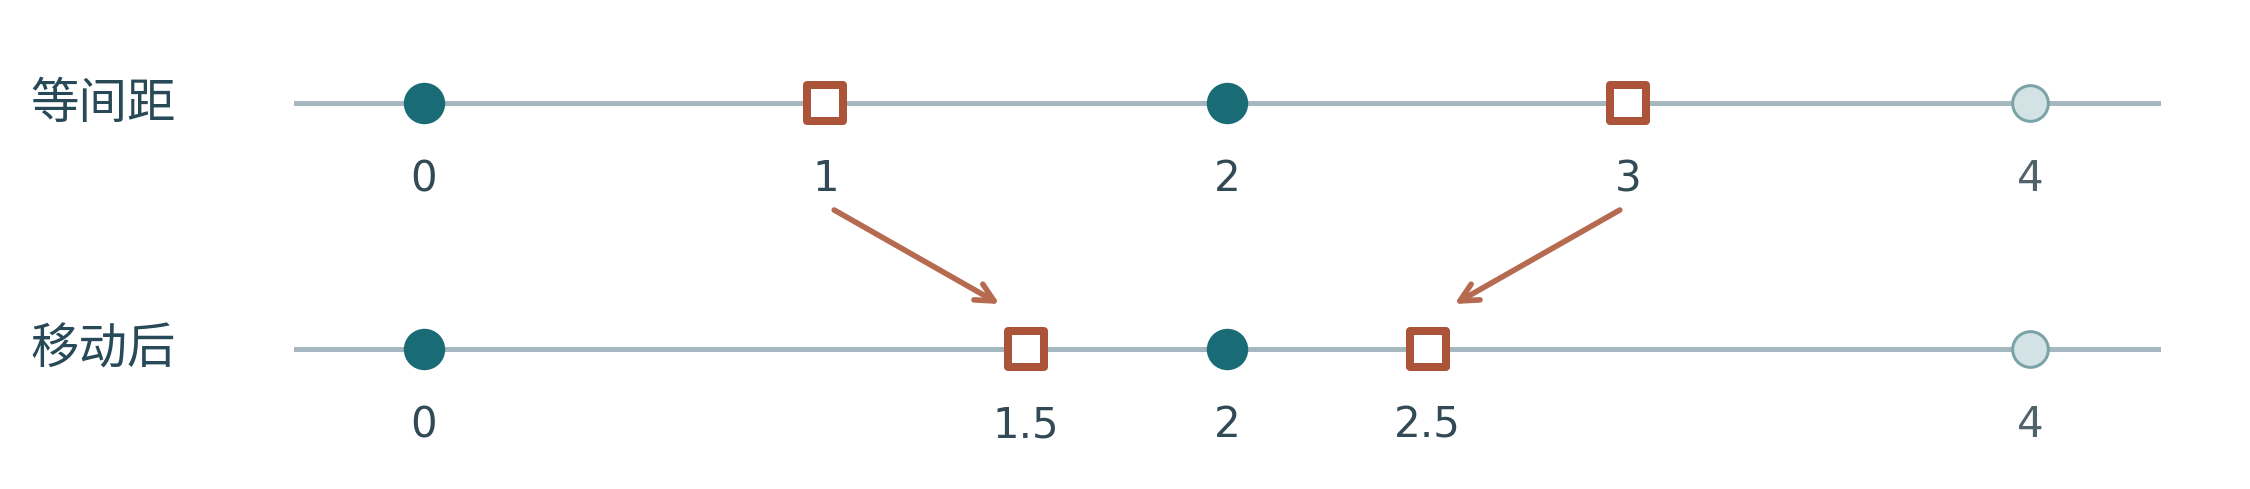
\includegraphics[width=.91\linewidth]{chain.png}\\[1mm]
{\small 图 1\quad 圆点为 A，方块为 B。横坐标 4 是下一周期的起点。}
\end{center}
\newpage
\section{每周期四个粒子的高斯势反例}
\begin{theorem}\label{thm:gauss}
取 $N=L=4$ 及 $f(r)=\exp(-r^2/4)$。若一个长度为四的周期内，粒子的位置为 $X=(0,3/2,2,5/2)$，则 $E_f(X)<E_f(U)$。
\end{theorem}
把通向下一个周期的间距也算在内，$X$ 的四个间距依次为 $3/2,1/2,1/2,3/2$。因此，两类粒子仍交替排列，密度为一，最小间距严格大于零。此外，$F(t)=e^{-t/4}$ 对每个整数 $k\ge0$ 均满足 $(-1)^k F^{(k)}(t)=4^{-k}e^{-t/4}>0$，故 $F$ 完全单调。

\begin{proof}
对 $f_a(r)=e^{-ar^2}$，令 $q=e^{-\pi^2/(16a)}$。由高斯函数的傅里叶变换可知，将 $f_a$ 按长度四周期化后，其第 $m$ 个傅里叶系数为 $(\sqrt{\pi/a}/4)q^{m^2}$，其中 $m\in\Z$。对所有粒子对求和，再扣除每个粒子与其自身的相互作用项，即得
\begin{align}
 E_{f_a}(Y)&=1-\frac{\sqrt{\pi/a}}{16}R(Y),\qquad
 R(Y)=\sum_{m\in\Z}q^{m^2}|S_m(Y)|^2,\label{eq:R}\\
 S_m(Y)&=\sum_{j=0}^3(-1)^j e^{i\pi m y_j/2}.\nonumber
\end{align}
实空间中的直接求和与傅里叶求和均绝对收敛。对等距构型，当 $m\equiv2\pmod4$ 时有 $|S_m(U)|=4$，其余各项均为零。对构型 $X$，$m=\pm1$ 两个模式的振幅平方均为 $2$。因此
\[
 R(X)\ge4q,\qquad R(U)=32\sum_{k\ge0}q^{(4k+2)^2}
          \le\frac{32q^4}{1-q^4}<4q\qquad(0<q\le1/4).
\]
最后一个不等式等价于 $8q^3+q^4<1$。特别地，取 $a=1/4$，便有 $q=e^{-\pi^2/4}<1/4$。式\eqref{eq:R}中 $R$ 的系数为负，故 $E_f(X)<E_f(U)$。
\end{proof}

直接求和得到 $U$ 的平均每粒子能量约为 $0.999633292158$，$X$ 的约为 $0.924751872822$。两者的严格大小关系已由上述不等式证明。把各自的四粒子单元重复若干次，即可对每个四的倍数 $N$ 得到相同的两组平均每粒子能量。若要求粒子靠近时相互作用势发散，可在 $f(r)$ 上加上 $\varepsilon r^{-2}$。由能量对势的线性关系和求和的绝对收敛性，只要 $\varepsilon>0$ 足够小，严格不等式仍成立。改变后的势作为距离平方的函数仍然完全单调。

\begin{proposition}\label{prop:instability}
令 $Y_s=(0,1+s,2,3-s)$，其中 $0<|s|<1$。对所有 $0<q\le1/4$，都有 $E_{f_a}(Y_s)<E_{f_a}(U)$。
\end{proposition}
\begin{proof}
由 $U$ 变为 $Y_s$，两个一阶谐波模式对 $R$ 的贡献合计增加 $8q\sin^2(\pi s/2)\ge8q s^2$。只有满足 $m\equiv2\pmod4$ 的模式，其贡献才可能减少。对这样的 $m$，有 $S_m(Y_s)=2+2\cos(\pi ms/2)$。利用 $16-(2+2\cos t)^2\le8t^2$，可知总减少量至多为
\[
  4\pi^2 s^2\sum_{m\ge2}m^2q^{m^2}
  \le \frac{16\pi^2 s^2q^4}{1-4q^2}.
\]
最后一步用到了 $m\ge2$ 时的两个不等式 $m^2\le4^{m-1}$ 和 $m^2\ge2m$。当 $0<q\le1/4$ 时，有 $2\pi^2q^3<1-4q^2$，所以上述上界严格小于 $8qs^2$。增量大于减量，再由式\eqref{eq:R}即得结论。
\end{proof}

\newpage
\section{指数核与任意正指数的里斯势}
\begin{theorem}\label{thm:exp}
令 $f_\kappa(r)=e^{-\kappa r}$，其中 $\kappa>0$，并记 $d_i=x_{i+1}-x_i$。则
\begin{equation}\label{eq:bound}
 E_{f_\kappa}(X)\ge1-\frac1N\sum_{i=0}^{N-1}
         \tanh(\kappa d_i/2)\ge1-\tanh(\kappa\ell/2)
         =E_{f_\kappa}(U).
\end{equation}
只有所有间距都相等时，能量才等于等距链的能量。对混合势 $f(r)=\int_{(0,\infty)}e^{-\kappa r}\dd\mu(\kappa)$，只要 $\mu$ 为非零正测度且每个 $r>0$ 都满足 $f(r)<\infty$，同一个等距构型也是唯一的能量最小构型。
\end{theorem}
\begin{proof}
将 $f_\kappa$ 周期化，得到 $K(t)=\sum_{n\in\Z}e^{-\kappa|t+nL|}$。定义
$Q=\sum_{ij}\sigma_i\sigma_j K(x_i-x_j)$，其中 $i,j$ 均遍历一个周期内的粒子。扣除 $N$ 个自身相互作用项后，$E_{f_\kappa}=1-Q/N$。在周长为 $L$ 的圆上，由格林函数恒等式 $(-\partial_t^2+\kappa^2)K=2\kappa\delta_0$ 可得
\[
 Q=\sup_{u\in H^1_{\rm per}(0,L)}
   \left\{2\sum_i\sigma_i u(x_i)-
    \frac1{2\kappa}\int_0^L\bigl((u')^2+\kappa^2 u^2\bigr)\dd t\right\}.
\]
对正定二次型配方可知，使上式取到上确界的场为 $u(t)=\sum_i\sigma_i K(t-x_i)$。现在考虑长度为 $d$ 的一个间隔，固定两端的场值 $v,w$，求此间隔上积分惩罚项的最小值。使其最小的函数满足 $u''=\kappa^2u$。计入系数 $1/(2\kappa)$ 后，最小值为
\[
 \tfrac14\bigl[\tanh(\kappa d/2)(v+w)^2+
             \coth(\kappa d/2)(v-w)^2\bigr].
\]
线性项可以恰好按相邻间隔分解成 $\sum_i\sigma_i(u(x_i)-u(x_{i+1}))$。为各个间隔分别取上界时，可以略去含 $(v+w)^2$ 的整个负项，再对 $v-w$ 配方。由此可知，长度为 $d$ 的间隔至多贡献 $\tanh(\kappa d/2)$。因此 $Q\le\sum_i\tanh(\kappa d_i/2)$。由于 $\tanh$ 在 $(0,\infty)$ 上严格凹，式\eqref{eq:bound}中的第二个不等式随之成立。若所有间距相等，对几何级数求和即得 $Q/N=1+2\sum_{m\ge1}(-e^{-\kappa\ell})^m=\tanh(\kappa\ell/2)$。

对混合势，任选向左或向右的一个方向，以 $r_j$ 表示参考粒子到该方向上第 $j$ 个邻居的距离。把求和项相邻配对，每一对的贡献 $f(r_{2j-1})-f(r_{2j})$ 均非负，且各对之和不超过 $f(r_1)$。这是因为 $f$ 单调递减，且支配收敛定理保证 $r\to\infty$ 时 $f(r)\to0$。对这些非负的成对项应用托内利（Tonelli）定理，得到 $E_f=\int E_{f_\kappa}\dd\mu(\kappa)$，其中能量有限。只要间距不全相等，对每个 $\kappa>0$，构型的能量就都严格大于等距链的能量。
\end{proof}

特别地，对每一个 $p>0$，均有
\[
r^{-p}=\frac{1}{\Gamma(p)}\int_0^\infty e^{-\kappa r}\kappa^{p-1}\dd\kappa.
\]
故等距链唯一达到最小能量
\[
E_f(U)=2\ell^{-p}\sum_{m\ge1}(-1)^{m+1}m^{-p}.
\]
上述配对论证使这一求和约定在 $0<p\le1$ 时仍然有据可依。由此可见，对距离 $r$ 完全单调的势构成一类，而对距离平方 $r^2$ 完全单调的势构成范围更广的一类。

\newpage
\paragraph{与尖界面模型已有结果的关系}
Giuliani、Lebowitz 和 Lieb\cite{GLL}研究了一维取值为 $\pm1$ 的场在指数核下的性质，以及给定磁化强度和跳跃次数时的简单周期能量极小构型。该结果与这里的估计可以直接联系起来。取周期阶梯场 $h$，使其满足 $h'=2\sum_i\sigma_i\delta_{x_i}$。在圆上分部积分得到 $4Q=2\kappa L-\kappa^2\langle h,K*h\rangle$，其中卷积和内积均按一个周期上的通常积分定义。Buttà 等人\cite{BEGM}在式（2.4）至（2.6）给出了分块估计以及周期块能量的显式表达式。将一个周期重复若干次，除以重复次数，再取极限，使每周期分摊的端点误差趋于零，即可得到式\eqref{eq:bound}的指数核不等式。因此，关于里斯势的结论是这一较早的尖界面不等式的推论。定理\ref{thm:exp}给出了直接从粒子变量出发的证明。本文的高斯势反例与能量界均供独立复核。

\subsection*{中文版附注：能量究竟降在了哪里？}
图 1 中只移动了 B 粒子。把无限链中的粒子对按物种拆开，可直接看出能量的增减。下表沿用式~\eqref{eq:energy} 的归一化；数值四舍五入至小数点后六位。
\begin{center}
\renewcommand{\arraystretch}{1.25}
\begin{tabular}{lrrr}
\hline
配对 & 等间距 & 移动后 & 能量变化 \\
\hline
A 与 A & $-0.386319$ & $-0.386319$ & $0$ \\
B 与 B & $-0.386319$ & $-0.461383$ & $-0.075065$ \\
A 与 B & $+1.772270$ & $+1.772454$ & $+0.000183$ \\
\hline
总计 & $0.999633$ & $0.924752$ & $-0.074881$ \\
\hline
\end{tabular}
\end{center}
原来相邻的 B 粒子相距 2，移动后，间距 1 和 3 交替出现。所有 B 与 B 的吸引合计使每粒子能量降低约 0.075065。每个 B 同时靠近一个 A、远离另一个 A；把整条链上的 A 都计入后，排斥能仅增加约 0.000183。两者相差约 409 倍。这个数值比较针对定理~\ref{thm:gauss} 所用的势宽、密度和位移。定理的严格证明见第 2 节。
\begin{thebibliography}{9}
\bibitem{BKN} L. Bétermin, H. Knüpfer and F. Nolte, Note on crystallization for alternating particle chains（关于交替粒子链结晶的札记）, \emph{J. Stat. Phys.} \textbf{181}, 803--815 (2020). \href{https://doi.org/10.1007/s10955-020-02603-2}{doi:10.1007/s10955-020-02603-2}.
\bibitem{GLL} A. Giuliani, J. L. Lebowitz and E. H. Lieb, Modulated phases of a one-dimensional sharp interface model in a magnetic field（磁场中一维尖界面模型的调制相）, \emph{Phys. Rev. B} \textbf{80}, 134420 (2009), 第 III 节. \href{https://doi.org/10.1103/PhysRevB.80.134420}{doi:10.1103/PhysRevB.80.134420}.
\bibitem{BEGM} P. Buttà, R. Esposito, A. Giuliani and R. Marra, Froth-like minimizers of a non-local free energy functional with competing interactions（具有竞争相互作用的非局域自由能泛函的泡沫状极小构型）, \emph{Commun. Math. Phys.} \textbf{323} (2013). \href{https://doi.org/10.1007/s00220-013-1740-z}{doi:10.1007/s00220-013-1740-z}.
\end{thebibliography}
\end{document}
